\chapter{Introducción específica} % Main chapter title

\label{Chapter2}

%----------------------------------------------------------------------------------------
%    SECTION 1
%----------------------------------------------------------------------------------------
En este capítulo se detallan las tecnologías utilizadas para el desarrollo del firmware, software y las plataformas necesarias para el funcionamiento del sistema.

\section{Centrales de alarma de incendio Simplex}
En los SDAI es común que los fabricantes incluyan un puerto para comunicación con dispositivos externos de registro de eventos, como por ejemplo impresoras. Estos puertos usualmente utilizan el protocolo RS232 \citep{rs232}, lo que hace posible registrar la información en un protocolo estándar en el ámbito industrial y de sistemas embebidos. En el caso de la marca Simplex, adicional a este puerto se incluye una terminal de comandos Telnet \citep{telnet} que obedece a un set de comandos. Esta interfaz sirve como herramienta de depuración durante la instalación de la CAI. Los comandos permiten confirmar elementos de programación tales como el accionamiento de los dispositivos de notificación, la ejecución del protocolo de evacuación, la información de todos los dispositivos instalados, y diversas funcionalidades avanzadas.

El uso de los comandos y su correcta interpretación requiere horas de capacitación y práctica, por lo que se podría considerar que existe una curva de aprendizaje considerable para el manejo de esta terminal. Esto se debe principalmente a que se requiere contar con conocimientos en diferentes aspectos del equipo como: el lenguaje de programación que utiliza, la nomenclatura del fabricante, el set de comandos de la marca, la estructura del programa en texto estructurado y la nomenclatura regulada de la NFPA, entre otros.  El acceso a este puerto suele recomendarse posterior a la segunda capacitación técnica oficial de la marca Simplex debido a su complejidad. En la figura \ref{fig:telnet} se puede observar un esquema que explica el funcionamiento del puerto.

\begin{figure}[ht]
   \centering
   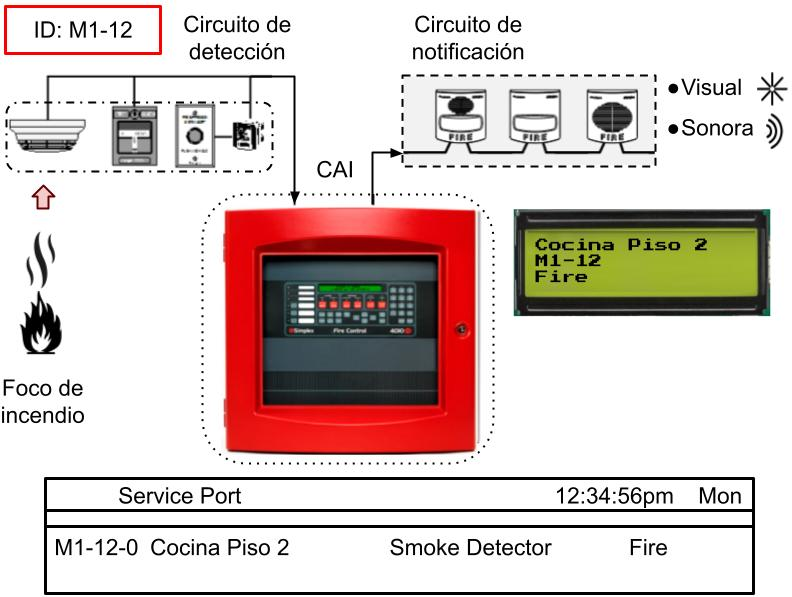
\includegraphics[scale=.45]{./Figures/telnet.jpg}
   \caption{Diagrama de notificaciones mediante puerto de servicio.}
   \label{fig:telnet}
\end{figure}


Considerando las características detalladas, el sistema actual se enfoca en el uso del puerto de comunicación Telnet para expandir los servicios a brindar por el SMAI. Al utilizar el puerto Telnet, se puede disponer de una plataforma que extraiga el detalle de los eventos de la central, y los facilite al usuario mediante Firebase. El objetivo principal es desarrollar un sistema de monitoreo de la CAI con el mayor detalle posible, pero a la vez es de especial interés facilitar el uso de esta plataforma para acelerar las tareas de instalación y mantenimiento de los SDAI Simplex.


\section{Sistema de monitoreo propuesto}

El sistema de monitoreo de alarma de incendio que se propone se compone de diferentes módulos. Como se puede observar en la figura \ref{fig:modulo}, cada módulo hace uso de una herramienta particular con los siguientes objetivos:

\begin{itemize}
\item \textit{Single Board Computer}: plataforma de desarrollo de hardware abierto con soporte para Linux embebido. Las plataformas utilizadas cuentan con soporte de sus comunidades, gran cantidad de tutoriales y documentación. \citep{bbb}.
\item Node-RED: herramienta de programación por bloques que permite la rápida integración de tecnologías y dispositivos. La herramienta permite integrar funcionalidades y servicios de forma sencilla, robusta y escalable. \citep{nodered}.
\item SQLite: biblioteca de funcionalidades que permite generar un motor de búsqueda SQL. El uso de bases de datos permite registrar la información de los eventos y generar un respaldo local de los eventos en caso de fallas de conexión a internet. \citep{sqlite}.
\item Firebase: plataforma enfocada en el desarrollo rápido de aplicaciones y servicios web que brinda un set completo de servicios. Permite incluir nuevas funcionalidades en pocos pasos y asegura la compatibilidad con todos los servicios suministrados por un mismo proveedor. \citep{fbase}.
\item Telegram: aplicación de mensajería que se utiliza como alternativa de notificación remota. Provee una estructura respaldada de mensajería instantánea que permite la notificación rápida al usuario.\citep{telegram}.
\end{itemize}


\begin{figure}[ht]
   \centering
   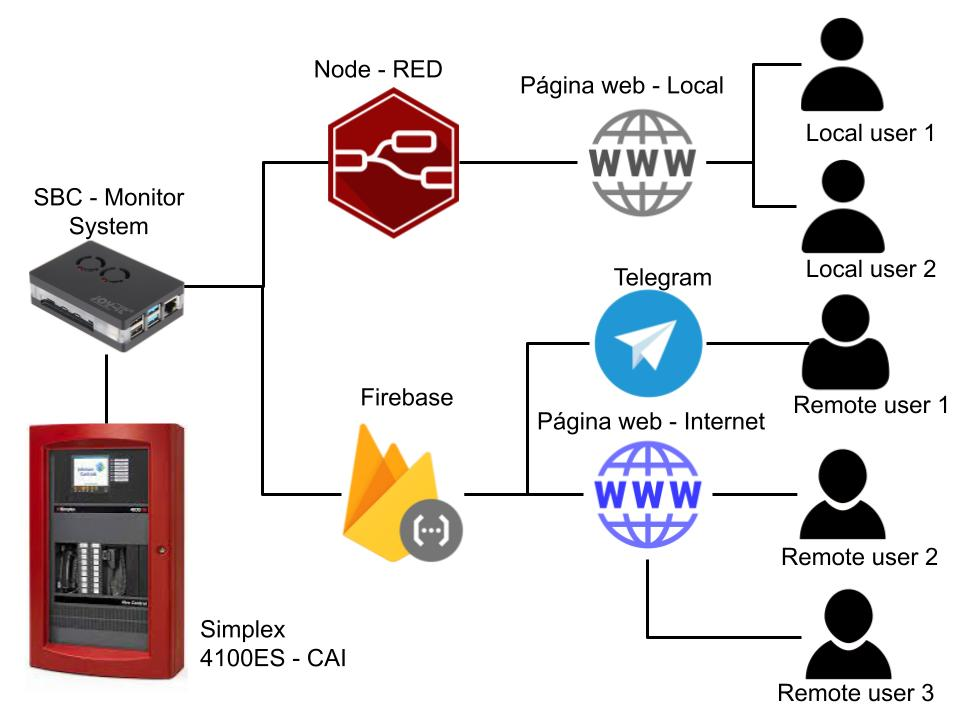
\includegraphics[scale=.35]{./Figures/modulo.jpg}
   \caption{Esquema resumido del sistema de monitoreo.}
   \label{fig:modulo}
\end{figure}


\section{Plataformas de desarrollo utilizadas}

\subsection{Plataforma de desarrollo web: Firebase}
Firebase es una plataforma alojada en la nube, que facilita el desarrollo de aplicaciones web y además integra diferentes servicios como:
\begin{itemize}
\item Autenticación: solución al control de acceso de usuarios, set de herramientas que gestionan el acceso de los usuarios de forma segura e incluso la recuperación de credenciales.
\item Base de datos en tiempo real: sistema de gestión de datos que facilita la sincronización de la información en todos los dispositivos con el acceso correspondiente.
\item Almacenamiento: servicio de almacenamiento de todo tipo de archivos. De gran utilidad para el intercambio de archivos como manuales, diagramas e ilustraciones por aprte del bot.
\item \textit{Hosting}: servicio que implementa y mantiene disponible las páginas web requeridas para el reporte de información mediante la web.
\item Funciones: servicio de ejecución de programas y automatizaciones configurables. Se utiliza para realizar el procesamiento de la información y la coordinación del reporte de eventos al resto de servicios.
\end{itemize}

La figura \ref{fig:d_fbase} muestra un esquema de los servicios de Firebase utilizados en el proyecto y su contribución. Los servicios más importantes a resaltar son el de funciones y la base de datos en tiempo real. Entre ambos servicios permiten incluir al sistema diferentes funcionalidades y coordinan los reportes de notificacion.

\begin{figure}[ht]
   \centering
   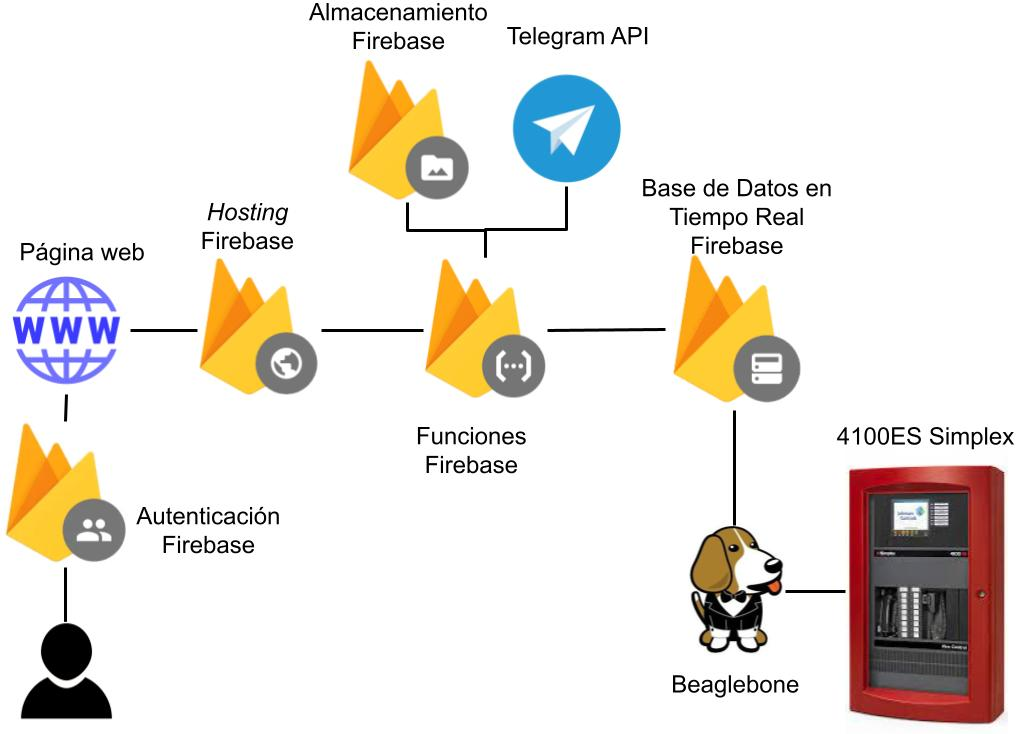
\includegraphics[scale=.35]{./Figures/d_fbase.jpg}
   \caption{Esquema de servicios de Firebase.}
   \label{fig:d_fbase}
\end{figure}



\subsection{Hardware de desarrollo}

En primera instancia, el sistema se continua en una Raspberry Pi 3 B + para el desarrollo de los programas, la interfaz de usuario, la validación de la estructura y el flujo de trabajo. Sin embargo, debido al feedback de expertos al finalizar el trabajo de investigación \citep{cese}.

Basados en la experiencia durante el cursado de la maestría se decide implementar el sistema en una placa Beaglebone Black \citep{bbb}, con el objetivo de incrementar la robustez del sistema y enfocar el desarrollo a un producto final. Adicional a las mejoras de hardware, también tenemos la posibilidad de compilar de forma cruzada nuestra propia versión de Linux con las características requeridas para el sistema.

\subsection{Herramienta de desarrollo de interfaz gráfica: Node-RED}

Herramienta de programación en bloque compatible con diferentes sistemas de bajo recursos. Simplifica la integración de dispositivos de hardware a través de módulos listos, que implementan los protocolos de comunicación más comunes en el ámbito industrial y de desarrollo. Además incluye módulos de generación de interfaces de usuario, que en pocos minutos establecen un servicio de hosting local con el objetivo de proveer un método de visualización y comando a partir de dispositivos con navegadores web. 

\subsection{Servicio de mensajería instantánea: Telegram}

Telegram corresponde al servicio de mensajería seleccionado para notificar a los usuarios de la presencia de un evento en su recinto. Telegram permite desarrollar de forma gratuita bots basados en su API, lo que brinda una atención más personalizada a los usuario y, adicionalmente, permite segmentar los servicios que proveen de forma clara. Si en dado caso se requiriera implementar nuevas funcionalidades, el esquema de trabajo de bots permite incorporar nuevas funcionalidades de forma sencilla, con la opción de habilitarlas sólo cuando estén funcionales y hayan sido testeadas correctamente.
